%% Chapter 13 — Version Control & Design History
%% Course 247-519-VA, Vanier College
%% Project Planning & Prototyping

\chapter{Version Control \& Design History}
\label{ch:version-control}

\paragraph{Where this fits.}
Chapter~12 delivered the cost analysis for the IoT robotic sorting subsystem --- unit cost at $N=50$, $100$, and $500$, break-even volume, and the economic case to proceed.
This chapter sits at the same Stage~3 (Development) gate, where those cost projections must be backed by an auditable design record.
Gate~3 requires a complete design package --- schematics, firmware, CAD models, BOM, and
test records --- that a reviewer (or a future team member) can evaluate, reproduce, and
certify.
A design package without a traceable history is not a package; it is a collection of files.
This chapter provides the tools and discipline to turn that collection into an auditable
record.

\paragraph{Learning Objectives.}
By the end of this chapter you will be able to:
\begin{enumerate}
  \item apply git branching, release tagging, and git-lfs configuration to a hardware design repository containing firmware, schematic, and CAD artifacts;
  \item write meaningful commit messages and manage branches for a hardware design project,
        including tagging milestone releases; and
  \item identify the purpose and required contents of a Design History File (DHF) and construct a DHF index that maps each required record category to its repository location.
\end{enumerate}

% ─────────────────────────────────────────────────────────────────────────────
\section{Why Version Control Matters for Hardware}
\label{sec:ch13-why}
% ─────────────────────────────────────────────────────────────────────────────

Software developers absorb version control as a survival skill early in their careers.
Hardware engineers have historically been slower to adopt it, partly because the dominant
artifacts --- schematics, PCB layouts, mechanical drawings --- are binary files that do not
diff cleanly, and partly because ``it worked yesterday'' is a powerful disincentive to
formalising a process that feels like overhead.

Both objections dissolve under Gate pressure.

\index{version control!hardware rationale}A change without a record is indistinguishable
from an error.
When a reviewer at Gate~3 finds that the BOM lists a 4.7~k$\Omega$ resistor and the
schematic shows a 10~k$\Omega$ resistor, there are exactly two possibilities: someone made
an unauthorised change, or a change was made and not recorded.
Without version history, the team cannot tell which.
Both outcomes are treated the same way by a certification auditor: as evidence of an
uncontrolled process.

\subsection{Design History as Design Evidence}
\label{subsec:ch13-history-is-evidence}

\index{design history!as evidence}In regulated industries (medical devices under ISO~13485,
aerospace under AS9100, automotive under IATF~16949), the \textbf{design history} is not
a nice-to-have supplement to the design; it is the design's proof of existence.
A product cannot be certified based on what it currently is; it is certified based on how
it got there --- what decisions were made, when, by whom, in response to what evidence.

Even outside regulated industries, the same logic applies at Gate~3 of a student project:
\begin{itemize}
  \item A reviewer asks, ``Why did you change the motor driver in Sprint~4?''
        Without a record, the answer is ``I think we had noise issues'' --- not defensible.
        With a version history, the answer is commit \texttt{b3c7a1f}: \emph{``fix(motor):
        replace DRV8833 with TB6612 to eliminate PWM-induced MQTT packet loss (see test log
        2026-04-28)''} --- citable, traceable, and credible.
  \item A teammate who joined mid-project needs to understand the current state without
        interrupting the rest of the team.
        The commit log is the onboarding document.
  \item Future you --- reproducing this design six months after submission --- has no memory
        of which firmware version ran during the Gate~3 demo.
        A release tag does.
\end{itemize}

\subsection{Scope: What Needs Version Control}
\label{subsec:ch13-scope}

\index{version control!scope}For the IoT robotic sorting subsystem, every artifact that
describes the design or its performance must be under version control:

\begin{itemize}
  \item \textbf{Firmware} --- all source files, build scripts, configuration headers, and
        dependency manifests (\texttt{CMakeLists.txt}, \texttt{platformio.ini},
        \texttt{requirements.txt}).
  \item \textbf{Schematics and PCB layouts} --- KiCad project files
        (\texttt{.kicad\_sch}, \texttt{.kicad\_pcb}), plus exported PDFs and Gerber
        archives as release artifacts.
  \item \textbf{CAD models} --- Fusion~360 version history internally; exported STEP and
        STL files committed as release artifacts.
  \item \textbf{Documentation} --- specifications (Chapter~4 artifact), BOM
        (Chapter~11 artifact), cost analysis (Chapter~12 artifact), test logs, and this
        chapter's DHF index.
\end{itemize}

% ─────────────────────────────────────────────────────────────────────────────
\section{Git for Firmware}
\label{sec:ch13-git-firmware}
% ─────────────────────────────────────────────────────────────────────────────

\index{git!firmware workflow}Students in this program already use git for software
coursework.
The discipline transfers directly to firmware; the differences are in commit granularity,
branching conventions, and the meaning of a release tag.

\subsection{Commit Discipline}
\label{subsec:ch13-commit-discipline}

\index{commit discipline}A commit is an atomic, self-contained unit of change accompanied
by a message that explains \emph{why} the change was made.
``WIP'' is not a commit message.
``Fixed stuff'' is not a commit message.
These messages carry zero information for future readers --- worse, they give the illusion that a record exists while providing none.

A well-formed commit message follows three rules:
\begin{enumerate}
  \item \textbf{Imperative mood subject line, $\leq$72 characters.}
        Write the subject as if completing the sentence ``If applied, this commit will\ldots''
        For example: ``add TLS client certificate authentication'' not ``added TLS'' or
        ``adding TLS.''
  \item \textbf{Type prefix.}
        A short prefix categorises the change: \texttt{feat} (new capability),
        \texttt{fix} (corrects a defect), \texttt{refactor} (restructures without
        changing behaviour), \texttt{docs} (documentation only), \texttt{test}
        (adds or updates tests), \texttt{chore} (tooling, CI, dependency bumps).
        This prefix lets a reviewer scan the log and immediately understand what category
        of change each commit represents.
  \item \textbf{Reference the evidence.}
        When a commit fixes a problem discovered during testing, name the test log or
        issue in the message body.
        ``\ldots (see test log 2026-04-28)'' turns a commit into a traceable decision
        record.
\end{enumerate}

\paragraph{Common Pitfalls.}
\begin{itemize}
  \item \textbf{``WIP'' as a commit message.}
        Work-in-progress commits are acceptable on a feature branch during development,
        but every commit that merges to \texttt{develop} or \texttt{main} must have a
        meaningful message.
        If your current practice is to commit with ``WIP'' and clean up later, use
        \texttt{git rebase -i} before merging to squash and rename those commits.
  \item \textbf{Committing for backup, not history.}
        Git is not Dropbox.
        A commit should represent a coherent state of the design, not merely the last
        save before leaving the lab.
        Separate ``save'' behaviour from ``history'' behaviour by using \texttt{git stash}
        for in-progress work and committing only when a logical unit is complete.
  \item \textbf{Giant commits.}
        A single commit that changes the schematic, three firmware modules, the BOM, and
        the README simultaneously cannot be reverted cleanly.
        Commit each logical change separately.
\end{itemize}

\subsection{Branching Strategy}
\label{subsec:ch13-branching}

\index{branching strategy}\index{git!branching}A branching strategy is a shared agreement
about which branches exist, what they contain, and how changes flow between them.
For a design project at Stage~3, a lightweight adaptation of the Gitflow model works well.
Figure~\ref{fig:ch13-git-flow} illustrates this branch structure with prototype milestones labelled.

\begin{figure}[htbp]
  \centering
  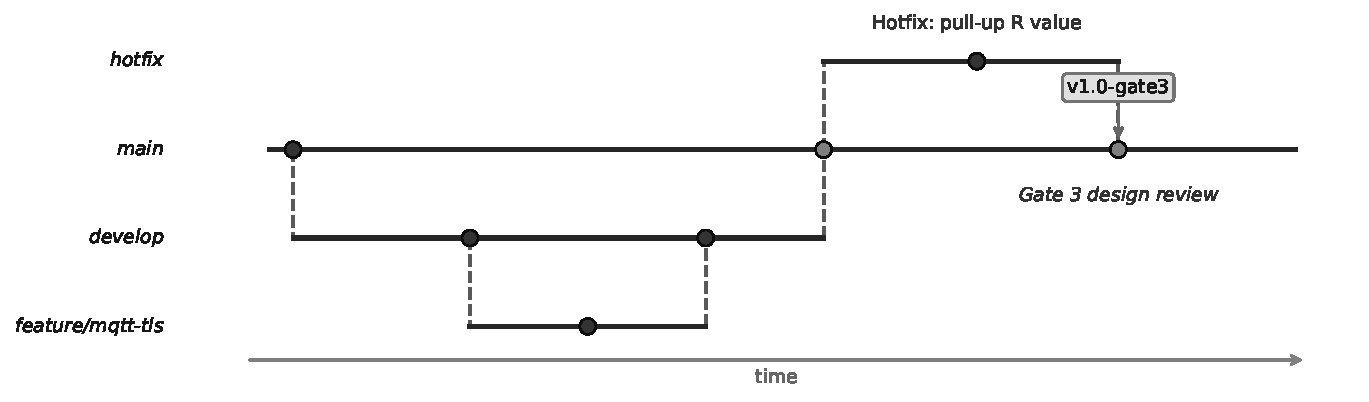
\includegraphics[width=0.92\textwidth]{chapters/13-version-control/images/fig_01_git_flow}
  \caption{Branch and merge diagram for the IoT robotic sorting subsystem design repository.
           The \texttt{main} branch carries only tagged, reviewed releases.
           Day-to-day integration happens on \texttt{develop}.
           Each new subsystem experiment opens a \texttt{feature/} branch that merges back
           to \texttt{develop} after team review.
           Emergency corrections after a milestone commit flow through a \texttt{hotfix/}
           branch directly to \texttt{main} and back to \texttt{develop}.}
  \label{fig:ch13-git-flow}
\end{figure}

The four branches have distinct roles:

\begin{itemize}
  \item \textbf{\texttt{main}} --- the golden branch.
        Every commit on \texttt{main} is a reviewed, tagged release.
        No one pushes directly to \texttt{main}; changes arrive only via a reviewed
        pull request or hotfix merge.
  \item \textbf{\texttt{develop}} --- the integration branch.
        This is where feature branches land after team review.
        It represents the current, buildable state of the design.
        Daily work happens here via merges from feature branches.
  \item \textbf{\texttt{feature/<name>}} --- subsystem experiment branches.
        When a team member is exploring an alternative sensor, a new MQTT library, or a
        mechanical bracket redesign, they work on a feature branch.
        This keeps half-finished experiments off \texttt{develop} while still providing
        version control for the experimental work.
        Examples: \texttt{feature/tls-auth}, \texttt{feature/tb6612-motor-driver},
        \texttt{feature/belt-bracket-v2}.
  \item \textbf{\texttt{hotfix/<name>}} --- post-release corrections.
        If a flaw is discovered after a Gate milestone tag, the fix branches from
        \texttt{main}, is applied minimally, and merges back to both \texttt{main}
        (with a new patch tag) and \texttt{develop} so the correction propagates forward.
\end{itemize}

\subsection{Tagging Releases}
\label{subsec:ch13-tagging}

\index{git!release tags}\index{release tag}A release tag marks a specific commit as a
named, reproducible state of the design.
Tags are not branches; they do not move as new commits are added.
For this course, the tagging convention is:

\begin{itemize}
  \item \texttt{v0.1-proto} --- first functional prototype, breadboard or perfboard stage.
  \item \texttt{v0.2-proto} --- iterated prototype, subsystems integrated.
  \item \texttt{v1.0-gate3} --- the design submitted for Gate~3 review; this tag freezes
        the exact state of every file the reviewer evaluates.
  \item \texttt{v1.1-post} --- post-Gate~3 hotfix, if a defect is discovered after
        submission.
\end{itemize}

Tagging the Gate~3 submission is not bureaucratic formality.
It means that six months from now, \texttt{git checkout v1.0-gate3} recovers the exact
design state the reviewer approved.
Without the tag, ``the version we submitted'' is ambiguous.

% ─────────────────────────────────────────────────────────────────────────────
\section{Worked Example: Five Commits from the Sorting Subsystem}
\label{sec:ch13-worked-example}
% ─────────────────────────────────────────────────────────────────────────────

The following git log covers three weeks of the IoT robotic sorting subsystem project,
from an early prototype build through the Gate~3 submission.
Read from bottom (oldest) to top (newest).

\begin{verbatim}
commit a1b2c3d (tag: v1.0-gate3, HEAD -> main)
Author: Team Sorter <team@example.com>
Date:   2026-05-15

    feat(mqtt): add TLS client certificate authentication

    Broker rejects unauthenticated connections per security review
    2026-05-12. Provisioned client cert from Let's Encrypt staging
    CA. See docs/security-review-2026-05-12.md.

commit f4e5d6c (origin/develop, develop)
Merge: 9d8e7f6 b1a2c3d
Author: Team Sorter <team@example.com>
Date:   2026-05-13

    Merge branch 'feature/tls-auth' into develop

    Reviewed by: J. Santos. All MQTT latency tests pass at <= 112 ms
    p99 after TLS handshake amortisation (see test log 2026-05-13).

commit b1a2c3d (feature/tls-auth)
Author: A. Kowalski <a.kowalski@example.com>
Date:   2026-05-10

    feat(mqtt): implement TLS 1.3 handshake on ESP32-S3

    Replaces plaintext MQTT with TLS 1.3 using mbedTLS bundled in
    ESP-IDF v5.2. Latency overhead measured at +18 ms p99 on first
    connect; amortised to +2 ms on subsequent publishes.

commit 9d8e7f6
Author: M. Tremblay <m.tremblay@example.com>
Date:   2026-04-28

    fix(motor): replace DRV8833 with TB6612 to eliminate
    PWM-induced MQTT packet loss

    DRV8833 switching noise at 20 kHz PWM caused Wi-Fi RF
    desensitisation (+6 dB noise floor on 2.4 GHz). TB6612 tested
    2026-04-27; packet loss dropped from 14% to <1%. BOM updated.
    See test log 2026-04-28.

commit 3c4d5e6 (tag: v0.1-proto)
Author: Team Sorter <team@example.com>
Date:   2026-04-20

    feat(sort): complete first-pass sensor + actuator integration

    Time-of-flight sensor (VL53L1X) and servo divert arm integrated
    on breadboard. Sort accuracy 91% over 50-item run. Known issue:
    PWM noise degrades Wi-Fi (tracked as issue #7).
\end{verbatim}

Before commit discipline was applied, these four changes were recorded as:
\texttt{WIP}, \texttt{update mqtt}, \texttt{fixed motor}, \texttt{done}.
None names the subsystem, none states the outcome, none cites evidence.
These messages are not archived history; they are noise.

\noindent\textbf{What this log demonstrates:}
\begin{itemize}
  \item Each commit message names a subsystem in parentheses, states an action in the
        imperative, and (in commits 2 and 4) cites a test log.
  \item The feature branch \texttt{feature/tls-auth} appears as three distinct commits ---
        the branch creation (implicit), the implementation commit, and the merge commit ---
        making the experiment's lifecycle visible in the log.
  \item Two release tags appear: \texttt{v0.1-proto} at first integration, and
        \texttt{v1.0-gate3} at the Gate~3 milestone.
  \item Commit \texttt{9d8e7f6} cross-references issue~\#7 opened in the
        \texttt{v0.1-proto} commit message, showing that a known defect was logged,
        tracked, and resolved --- the essence of a controlled design process.
\end{itemize}

\subsubsection{Reconstructing Design State at Any Commit}
\label{subsubsec:ch13-checkout}

\index{git!checkout historical state}The most powerful property of a commit log is
reproducibility.
To recover the exact state of the sorter firmware, schematic, and documentation as it
stood at the \texttt{v0.1-proto} tag:

\begin{verbatim}
git checkout v0.1-proto
\end{verbatim}

\noindent Git places the working tree in a ``detached HEAD'' state at that commit.
Every file is exactly as it was when that commit was recorded --- including the BOM, the
firmware, and any exported PDFs committed alongside the source.
To inspect the state at an arbitrary commit hash:

\begin{verbatim}
git checkout 9d8e7f6
\end{verbatim}

\noindent To return to the current \texttt{main}:

\begin{verbatim}
git checkout main
\end{verbatim}

\noindent This capability is what converts a repository from a backup system into a design
history: the ability to answer ``exactly what was the design on 2026-04-28?'' with a
single command.

% ─────────────────────────────────────────────────────────────────────────────
\section{Version Control for Design Files}
\label{sec:ch13-design-files}
% ─────────────────────────────────────────────────────────────────────────────

\index{version control!design files}Firmware is plain text; git handles it natively.
Schematic, PCB, and CAD files range from structured text (KiCad's native format) to
proprietary binary (older ECAD tools, Fusion~360 native files).
Each category requires a slightly different approach.

\subsection{EDA Files: KiCad and Git}
\label{subsec:ch13-kicad}

\index{KiCad!git integration}\index{EDA version control}KiCad~7 and later store schematics
(\texttt{.kicad\_sch}) and PCB layouts (\texttt{.kicad\_pcb}) as structured text files
(S-expression format).
These files diff legibly --- a net renamed, a footprint repositioned, or a trace re-routed
produces a human-readable diff.
KiCad projects belong in the git repository alongside firmware.

A recommended KiCad project layout within the repository:

\begin{verbatim}
hardware/
  sorter-pcb/
    sorter-pcb.kicad_pro
    sorter-pcb.kicad_sch
    sorter-pcb.kicad_pcb
    fp-lib-table
    sym-lib-table
    exports/
      sorter-pcb-schematic-v1.0.pdf
      gerbers-v1.0/
\end{verbatim}

The \texttt{exports/} subdirectory holds generated artifacts committed at each release
milestone.
Reviewers receive the PDF; the source files allow regeneration.

A \texttt{.gitignore} for a KiCad project should exclude autogenerated files that change
on every open:

\begin{verbatim}
# KiCad autogenerated
*.kicad_prl
*-backups/
fp-info-cache
\end{verbatim}

\subsection{CAD Files: Fusion 360 and STEP Exports}
\label{subsec:ch13-cad}

\index{Fusion 360!version history}\index{CAD version control}\index{STEP export}Fusion~360
maintains its own cloud version history per design --- every save creates a numbered version
accessible from the timeline panel.
This internal history is not a git repository, but it provides equivalent capability for
pure mechanical work: named versions, rollback, and branch-like ``branch design'' features.

For the purposes of the DHF and Gate~3 package, the key practice is exporting milestone
versions as \textbf{STEP files} (\texttt{.step}) and committing them to the repository:

\begin{verbatim}
hardware/
  sorter-chassis/
    exports/
      sorter-chassis-v0.1-proto.step
      sorter-chassis-v1.0-gate3.step
\end{verbatim}

STEP is a neutral, open exchange format readable by any CAD tool.
Committing STEP exports ensures that the Gate~3 package contains manufacturable geometry
even if the original Fusion~360 licence expires or the cloud account is unavailable.

\subsection{Binary Files and Git LFS}
\label{subsec:ch13-lfs}

\index{git-lfs}\index{Git Large File Storage}Git stores file history by retaining every
version of every file.
For large binary files --- Gerber archives, STEP models, compiled firmware binaries,
rendered images --- this causes repository bloat: cloning the repository downloads every
historical version of every binary, which can quickly reach hundreds of megabytes.

\textbf{Git Large File Storage (git-lfs)} solves this by replacing large binaries in the
repository with small pointer files, while storing the actual binary content on a
compatible server (GitHub LFS, GitLab LFS, or a self-hosted server).
Only the versions actually checked out are downloaded.

Setup requires two steps, run once per repository:

\begin{verbatim}
git lfs install
git lfs track "*.step" "*.pdf" "*.zip" "*.bin"
git add .gitattributes
git commit -m "chore: configure git-lfs for binary design artifacts"
\end{verbatim}

The \texttt{git lfs track} command adds patterns to \texttt{.gitattributes}.
All team members must have git-lfs installed; cloning without it produces pointer-file
stubs instead of actual content.

\paragraph{Common Pitfalls.}
\begin{itemize}
  \item \textbf{Committing binary blobs without LFS.}
        Adding a 15~MB Gerber ZIP to git without LFS embeds that 15~MB permanently in the
        repository history.
        \texttt{git rm} does not help; the blob persists in every future clone.
        Removing it requires rewriting history with \texttt{git filter-branch} or the
        BFG Repo Cleaner, which disrupts all collaborators.
        Configure LFS \emph{before} committing any binary artifact.
  \item \textbf{Tracking every file type with LFS.}
        KiCad \texttt{.kicad\_sch} and \texttt{.kicad\_pcb} files are structured text
        and should \emph{not} go through LFS --- their diffs are the most valuable part
        of the schematic history.
        Only true binaries and large generated outputs belong in LFS.
\end{itemize}

% ─────────────────────────────────────────────────────────────────────────────
\section{The Design History File}
\label{sec:ch13-dhf}
% ─────────────────────────────────────────────────────────────────────────────

\index{Design History File}\index{DHF}The \textbf{Design History File (DHF)} is the
auditable record of all design decisions, changes, approvals, and test results associated
with a product.
In regulated product development, the DHF is a formal document set required for
certification; a product without a DHF cannot be cleared, approved, or certified.

In this course, the \textbf{portfolio is the DHF}.
Every artifact produced across Chapters~1 through~14 --- the central question, the
specification, the risk register, the architecture diagram, the BOM, the cost analysis, and
the test records --- collectively constitutes the design history.
The DHF index page produced in this chapter is the document that proves those artifacts
exist, locates them in the repository, and shows that they are current.

\subsection{Required Contents of a DHF}
\label{subsec:ch13-dhf-contents}

\index{DHF!required contents}A complete DHF contains four categories of records. Figure~\ref{fig:ch13-dhf-structure}, shown after the list, illustrates how these records feed the Gate~3 package.

\begin{enumerate}
  \item \textbf{Design records} --- the specification (Chapter~4), architecture diagram
        (Chapter~5), schematic and PCB files, CAD models, firmware source, and BOM
        (Chapter~11).
        These describe \emph{what the design is}.
  \item \textbf{Test records} --- bench test logs, latency characterisation results,
        accuracy trial data, environmental tests.
        These describe \emph{what was observed}.
  \item \textbf{Change records} --- Engineering Change Orders (Section~\ref{sec:ch13-eco})
        or, in this course, annotated git commit messages and merge records.
        These describe \emph{what changed and why}.
  \item \textbf{Approval records} --- peer review sign-offs, instructor feedback records,
        and Gate decision documents.
        These describe \emph{who reviewed and accepted each change}.
\end{enumerate}

\begin{figure}[htbp]
  \centering
  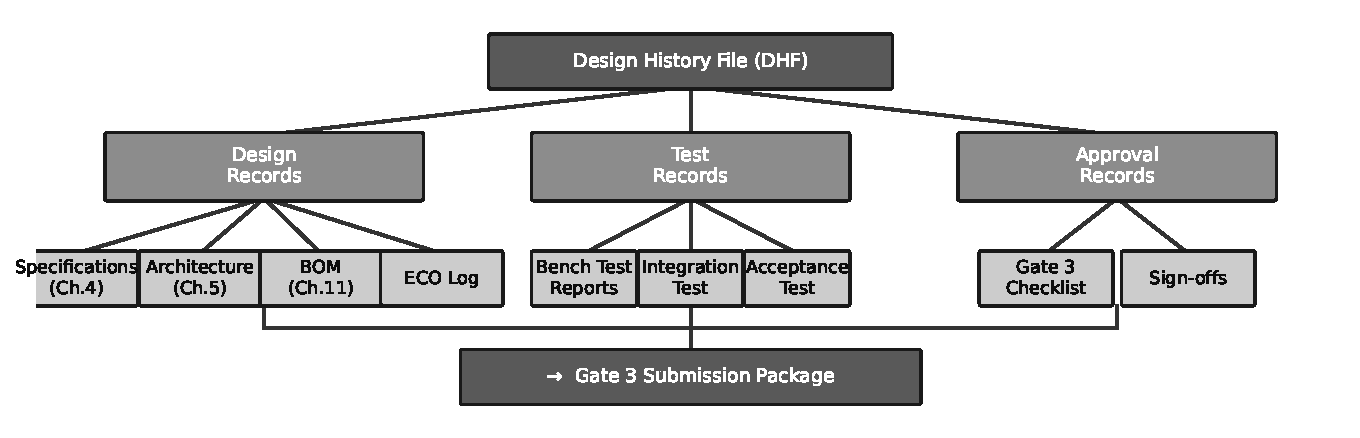
\includegraphics[width=0.88\textwidth]{chapters/13-version-control/images/fig_02_dhf_structure}
  \caption{The Design History File as a tree of records feeding into the Gate~3 document.
           Design records capture what was decided; test records capture what was observed;
           change records capture what was modified and why; approval records capture who
           reviewed and accepted each change.
           Together they form the traceable chain of evidence required for Gate~3.}
  \label{fig:ch13-dhf-structure}
\end{figure}

\subsection{The DHF Index}
\label{subsec:ch13-dhf-index}

\index{DHF!index}The DHF index is a single document --- typically a Markdown or \LaTeX{}
file at the root of the repository --- that maps each required record to its location.
Its purpose is navigation: a reviewer should be able to open the index and locate any
specific record within two clicks or two commands.

A minimal DHF index for the sorting subsystem project:

\begin{verbatim}
# Design History File Index — IoT Robotic Sorting Subsystem
# Gate 3 Submission: tag v1.0-gate3 (2026-05-15)

## Design Records
- Specification (REQ-01 to REQ-05):
    docs/specification.md  (commit 3c4d5e6)
- Architecture diagram:
    docs/architecture.pdf  (commit 7a8b9c0)
- Schematic (KiCad):
    hardware/sorter-pcb/sorter-pcb.kicad_sch
- BOM v1.0:
    hardware/bom-v1.0.csv  (commit e2f3a4b)
- Firmware source:
    firmware/src/          (tag v1.0-gate3)

## Test Records
- MQTT latency characterisation (2026-05-13):
    docs/test-logs/mqtt-latency-2026-05-13.md
- Sort accuracy trial, 100-item run (2026-05-08):
    docs/test-logs/sort-accuracy-2026-05-08.md

## Change Records
- Motor driver substitution (DRV8833 -> TB6612):
    git log 9d8e7f6
- TLS authentication addition:
    git log b1a2c3d

## Approval Records
- Gate 3 review:
    docs/gate3-review-2026-05-16.md
\end{verbatim}

Every entry names the file and the commit or tag at which that file was current.
A future reviewer can \texttt{git checkout} the named commit and retrieve the exact version
of each record that was present at Gate~3.

\paragraph{In Practice.}
Teams who maintain the DHF index throughout the project --- updating it whenever a new
artifact is produced --- find Gate~3 preparation trivial: the index already exists, the
records are already filed, and the submission is a matter of tagging the repository and
attaching the index.
Teams who leave the DHF index for the last week before Gate~3 discover that they cannot
locate test logs, cannot match BOM versions to schematic revisions, and cannot reconstruct
the decision trail that led to the current design.
The DHF is not preparation for Gate~3; it is the continuous record that makes Gate~3
possible.

% ─────────────────────────────────────────────────────────────────────────────
\section{Change Management}
\label{sec:ch13-eco}
% ─────────────────────────────────────────────────────────────────────────────

\index{change management}\index{engineering change order}\index{ECO}Every design changes
during development.
The question is not whether changes will happen but whether they will be recorded.
Change management is the discipline of deciding, for each change, whether it requires a
formal record and, if so, ensuring that record is created.

\subsection{Informal Fix vs.\ Formal ECO}
\label{subsec:ch13-informal-vs-formal}

\index{ECO!informal vs.\ formal}Not every change requires an Engineering Change Order.
A typo correction in a comment, a cosmetic alignment fix in a schematic, or a variable
rename in firmware can be committed directly with an appropriate message.
The decision threshold is whether the change affects form, fit, or function:

\begin{itemize}
  \item \textbf{Form} --- physical dimensions, connector locations, mounting hole patterns.
  \item \textbf{Fit} --- how the component or assembly interfaces with adjacent parts.
  \item \textbf{Function} --- what the system does, including electrical characteristics,
        software behaviour, or communication protocol parameters.
\end{itemize}

Any change that affects form, fit, or function in a way that could alter test results or
require retesting triggers a formal change record.
Figure~\ref{fig:ch13-eco-flow} maps this decision.

\begin{figure}[htbp]
  \centering
  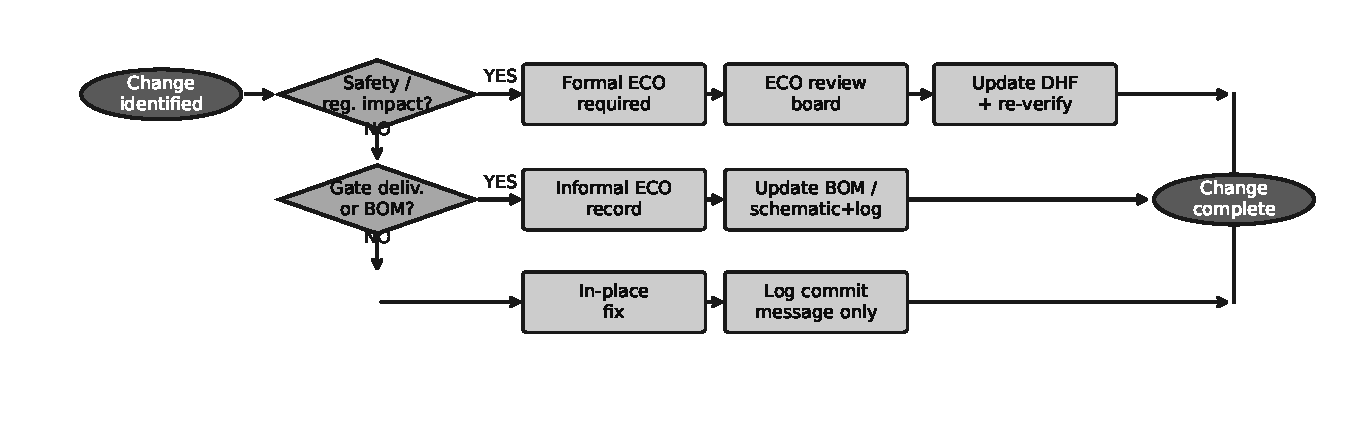
\includegraphics[width=0.80\textwidth]{chapters/13-version-control/images/fig_03_eco_flow}
  \caption{Engineering change order decision flow.
           Changes that do not affect form, fit, or function proceed as a standard commit.
           Changes that affect form, fit, or function require a documented rationale and,
           if the design is post-release (past a Gate milestone tag), a formal ECO with
           reviewer sign-off before implementation.}
  \label{fig:ch13-eco-flow}
\end{figure}

\subsection{The ECO in Practice}
\label{subsec:ch13-eco-practice}

\index{ECO!contents}A formal Engineering Change Order contains:
\begin{enumerate}
  \item \textbf{Change ID and date} --- a unique identifier (e.g., ECO-003) and the date
        the change was initiated.
  \item \textbf{Description of the change} --- what is being changed, from what to what,
        in each affected artifact (schematic, firmware, BOM, documentation).
  \item \textbf{Reason for the change} --- the evidence or observation that motivated it
        (test log reference, defect report, customer feedback, new component availability).
  \item \textbf{Impact assessment} --- which other subsystems, tests, or documents are
        affected; whether retesting is required.
  \item \textbf{Approval} --- who authorised the change; date authorised.
  \item \textbf{Implementation reference} --- the git commit hash or tag at which the
        change was applied.
\end{enumerate}

In this course, the ECO is implemented as a short Markdown file committed to
\texttt{docs/eco/ECO-003.md} with the above fields.
The git commit that implements the change references the ECO number in its message:
\texttt{fix(motor): replace DRV8833 per ECO-003}.

\paragraph{In Practice.}
A team made a last-minute resistor value change without recording it.
The prototype passed testing, went to Gate~3, and the reviewer asked why the BOM listed
4.7~k$\Omega$ and the schematic showed 10~k$\Omega$.
No one could answer.
The change had been made on the bench during a late-night session, the schematic was not
updated, and no commit was made.
From the reviewer's perspective, the design was incoherent: the BOM and schematic described
two different circuits.
An ECO process --- or even a committed git message reading \emph{``fix(adc-bias): change
R12 from 10k to 4.7k to correct voltage divider for 3.3V ADC reference (see
test-log-2026-05-09)''} --- would have caught this.
A 60-second commit prevents a Gate-day crisis.

% ─────────────────────────────────────────────────────────────────────────────
\section{Practical Tooling}
\label{sec:ch13-tooling}
% ─────────────────────────────────────────────────────────────────────────────

\index{tooling!version control}This section summarises the tool stack for the sorting
subsystem project and provides configuration guidance.

\subsection{Git and GitHub/GitLab}
\label{subsec:ch13-git-platforms}

\index{GitHub}\index{GitLab}The repository should be hosted on a platform that supports:
\begin{itemize}
  \item \textbf{Pull requests / merge requests} --- the mechanism for team code review
        before merging feature branches to \texttt{develop}.
  \item \textbf{Issues} --- the lightweight defect and task tracker; commit messages
        reference issue numbers (\texttt{closes \#7}).
  \item \textbf{Git LFS} --- large binary storage; both GitHub and GitLab offer LFS
        storage with free-tier quotas sufficient for a student project.
  \item \textbf{Releases} --- GitHub and GitLab both surface git tags as named releases
        with attached assets; tagging \texttt{v1.0-gate3} automatically populates the
        Releases page, providing a clean download link for the Gate~3 submission package.
\end{itemize}

A recommended repository root structure for the sorter project:

\begin{verbatim}
sorter-project/
  firmware/
    src/
    include/
    platformio.ini
  hardware/
    sorter-pcb/         (KiCad project)
    sorter-chassis/
      exports/          (STEP, STL)
  docs/
    specification.md
    architecture.pdf
    bom-v1.0.csv
    test-logs/
    eco/
    dhf-index.md
  .gitattributes        (git-lfs patterns)
  .gitignore
  README.md
\end{verbatim}

\subsection{KiCad Git Integration}
\label{subsec:ch13-kicad-git}

\index{KiCad!version control}KiCad~7's native file format is git-friendly by design.
The recommended workflow:

\begin{enumerate}
  \item Open the KiCad project folder as the git working directory (not as a subdirectory
        of a larger project with unrelated files).
  \item Add the \texttt{.gitignore} exclusions for \texttt{*.kicad\_prl} and
        \texttt{*-backups/} (KiCad autogenerates these on every open).
  \item Commit schematic and PCB changes separately from firmware changes.
        A single commit that mixes a schematic net change with a firmware fix is harder to
        review and harder to revert.
  \item Export schematic PDF and BOM CSV at each release milestone and commit them to
        \texttt{hardware/sorter-pcb/exports/} before tagging.
\end{enumerate}

\subsection{Fusion 360 Version History}
\label{subsec:ch13-fusion360}

\index{Fusion 360!version history}Fusion~360 saves version history to Autodesk cloud
storage automatically on each save.
Each version can be named (\texttt{v0.1-proto-belt-bracket}, \texttt{v1.0-gate3-chassis})
from the Version History panel.
This naming should mirror the git tag convention so that a reviewer can correlate the
mechanical version with the corresponding firmware and schematic commit.

The synchronisation point is the STEP export committed to the git repository at each
release tag.
The process:
\begin{enumerate}
  \item In Fusion~360, name the current version to match the planned git tag
        (e.g., \texttt{v1.0-gate3}).
  \item Export as STEP: \texttt{File > Export > STEP (.step)}.
  \item Place the STEP file in \texttt{hardware/sorter-chassis/exports/} and commit it
        to git with the message \texttt{chore(cad): export v1.0-gate3 STEP for DHF}.
  \item Tag the repository: \texttt{git tag -a v1.0-gate3 -m "Gate 3 submission"}.
\end{enumerate}

\subsection{Keeping the DHF in the Repository}
\label{subsec:ch13-dhf-in-repo}

\index{DHF!repository integration}The DHF index (\texttt{docs/dhf-index.md}) lives in the
same repository as the design.
This means:
\begin{itemize}
  \item The DHF is versioned alongside the design it documents.
  \item \texttt{git checkout v1.0-gate3} retrieves the DHF index as it stood at Gate~3
        submission, listing the exact file versions that were current at that moment.
  \item There is no separate document management system to synchronise; the repository
        \emph{is} the document management system.
\end{itemize}

% ─────────────────────────────────────────────────────────────────────────────
\section*{Try It Yourself}
\addcontentsline{toc}{section}{Try It Yourself}
\label{subsec:ch13-try-it}
% ─────────────────────────────────────────────────────────────────────────────

\begin{quote}
\textbf{Scenario:} A team is developing a \textbf{smart aquarium controller} that monitors
water temperature, pH, and turbidity, controls a heating element and a peristaltic dosing
pump, and publishes sensor readings to a local MQTT broker over Wi-Fi.
Their git log for the most recent four commits reads:

\begin{verbatim}
commit d4e5f6a (HEAD -> main)
Author: Aqua Team <aqua@example.com>
Date:   2026-05-10

    stuff

commit 9b8c7d6
Author: Aqua Team <aqua@example.com>
Date:   2026-05-09

    WIP sensor code

commit 1a2b3c4
Author: Aqua Team <aqua@example.com>
Date:   2026-05-07

    update

commit 5e6f7a8
Author: Aqua Team <aqua@example.com>
Date:   2026-05-03

    feat(temp): add DS18B20 one-wire temperature sampling at 1 Hz

    Sampling loop validated against NIST-traceable reference
    thermometer; error < 0.2 degC across 15-35 degC range.
    See test-log-2026-05-03.md.
\end{verbatim}

\textbf{Your tasks:}
\begin{enumerate}
  \item Identify which commits have poorly written messages and explain specifically what
        information is missing from each.
  \item Rewrite the three poorly written commit messages following the type-prefix,
        imperative mood, and evidence-citation conventions introduced in
        Section~\ref{subsec:ch13-commit-discipline}.
        Use plausible content consistent with the aquarium controller context.
        Do not invent test results; instead reference a test log by filename.
  \item The team has a STEP export of their sensor bracket committed without git-lfs (\texttt{sensor-bracket.step}, 22~MB). Address the following:
  \begin{enumerate}
    \item[(a)] How to prevent future large files from bypassing LFS.
    \item[(b)] Why the existing 22~MB blob cannot be removed with \texttt{git rm} alone and what tool is required.
  \end{enumerate}
  \item Sketch (in plain text or a simple diagram) a DHF index for the aquarium controller
        at a Gate~3 milestone, listing at least one entry in each of the four DHF
        categories from Section~\ref{subsec:ch13-dhf-contents}.
\end{enumerate}
\end{quote}

% ─────────────────────────────────────────────────────────────────────────────
\section*{Review Questions}
\addcontentsline{toc}{section}{Review Questions}
\label{sec:ch13-review}
% ─────────────────────────────────────────────────────────────────────────────

\begin{enumerate}

  \item \textbf{(Conceptual)} Explain the statement ``a change without a record is
        indistinguishable from an error.''
        A team's prototype passes all Gate~3 bench tests, but the reviewer flags a
        discrepancy between the BOM and the schematic.
        What two possibilities does the reviewer face, and why can the team not resolve the
        ambiguity without version history?

  \item \textbf{(Conceptual)} Compare the roles of the \texttt{develop} branch and the
        \texttt{main} branch in the Gitflow branching strategy described in this chapter.
        Why should direct pushes to \texttt{main} be prohibited, and what mechanism should
        be used instead?

  \item \textbf{(Applied)} The following four commit messages appear in a project
        repository.
        For each, state whether it is acceptable or poor, and if poor, rewrite it following
        the conventions in Section~\ref{subsec:ch13-commit-discipline}.
        \begin{enumerate}
          \item[(a)] \texttt{WIP}
          \item[(b)] \texttt{feat(lidar): add VL53L1X ranging loop with 50~ms sampling interval, validated against tape-measure reference over 0.1--2.0~m (see test-log-2026-04-15.md)}
          \item[(c)] \texttt{fixed the thing}
          \item[(d)] \texttt{updated files}
        \end{enumerate}

  \item \textbf{(Applied)} A teammate commits a 40~MB Gerber ZIP file to the repository
        without git-lfs.
        \begin{enumerate}
          \item[(a)] Explain why \texttt{git rm gerbers.zip \&\& git commit} does not
                     reduce the repository size for new clones.
          \item[(b)] Describe the correct remediation steps, including which external tool
                     is commonly used to rewrite repository history and what the
                     operational consequence is for all other team members after the
                     history rewrite.
          \item[(c)] State the \texttt{git lfs track} command that would have prevented
                     this problem for all future ZIP files.
        \end{enumerate}

  \item \textbf{(Multi-step --- conceptual + applied)} A team completes Gate~3.
        One week later, a reviewer discovers that the pulse-width modulation frequency
        used in the actuator firmware was changed from 20~kHz to 10~kHz during the final
        sprint but does not appear in any commit message, the BOM, the schematic, or the
        DHF index.
        \begin{enumerate}
          \item[(a)] Identify which of the four DHF record categories
                     (Section~\ref{subsec:ch13-dhf-contents}) is missing for this change.
          \item[(b)] Describe how an ECO record, had it been created, would have captured
                     this change, naming the six fields from
                     Section~\ref{subsec:ch13-eco-practice}.
          \item[(c)] Explain whether the existing \texttt{v1.0-gate3} tag can be used to
                     reconstruct the state of the firmware at Gate~3 submission, and what
                     additional step would now be required to document the discrepancy
                     without destroying the Gate~3 record.
        \end{enumerate}

\end{enumerate}

% ─────────────────────────────────────────────────────────────────────────────
\section*{Portfolio Entry}
\addcontentsline{toc}{section}{Portfolio Entry}
\label{sec:ch13-artifact}
% ─────────────────────────────────────────────────────────────────────────────

This chapter produces two linked deliverables that together constitute the version-control
component of your Gate~3 package:

\begin{enumerate}
  \item \textbf{Git repository with a meaningful commit log.}
        Your project repository on GitHub or GitLab must contain:
        \begin{enumerate}
          \item[(a)] A \texttt{main}/\texttt{develop}/\texttt{feature} branch structure
                     consistent with the strategy in Section~\ref{subsec:ch13-branching}.
          \item[(b)] At least five commits with meaningful messages following the
                     type-prefix and imperative-mood conventions, covering the design
                     period from your first prototype integration to Gate~3.
          \item[(c)] At least one feature branch that was created for a subsystem
                     experiment and merged back to \texttt{develop} via a pull request.
          \item[(d)] A release tag \texttt{v1.0-gate3} applied to the commit that
                     represents your Gate~3 submission state.
        \end{enumerate}

  \item \textbf{DHF index page.}
        A file \texttt{docs/dhf-index.md} committed to the repository at the
        \texttt{v1.0-gate3} tag, containing:
        \begin{enumerate}
          \item[(a)] At least one entry in each of the four DHF record categories
                     (design records, test records, change records, approval records).
          \item[(b)] For each entry: the filename (relative to the repository root),
                     the git commit hash or tag at which that file was current, and a
                     one-line description of the record's content.
          \item[(c)] The full command required to reproduce the Gate~3 submission state:
                     \texttt{git checkout v1.0-gate3}.
        \end{enumerate}
\end{enumerate}

% ─────────────────────────────────────────────────────────────────────────────
\section*{Chapter Summary}
\addcontentsline{toc}{section}{Chapter Summary}
\label{sec:ch13-summary}
% ─────────────────────────────────────────────────────────────────────────────

A design without version control is not under control; it is under the assumption that
nothing will go wrong.
This chapter established three interlocking disciplines.

First, every design artifact --- firmware, schematic, PCB layout, CAD model, BOM, and
documentation --- belongs in a version-controlled repository.
Design history is design evidence: reviewers certify not what a product currently is, but how it got there.

Second, commit discipline and branching strategy are not software-only concerns.
Meaningful commit messages in imperative mood with type prefixes and evidence citations
turn a git log into a design decision trail.
The \texttt{main}/\texttt{develop}/\texttt{feature} branch structure keeps experimental
work isolated until it is reviewed and ready to integrate.
Release tags --- \texttt{v0.1-proto}, \texttt{v1.0-gate3} --- freeze exact design states
that can be recovered with a single \texttt{git checkout} command.

Third, the Design History File is not a document produced at the end of a project; it is a
continuous record maintained throughout the project.
The DHF index maps design records, test records, change records, and approval records to
their repository locations.
The ECO process --- deciding whether a change affects form, fit, or function, and recording
it if it does --- is the mechanism that keeps the DHF current.
A 60-second commit referencing a test log prevents the Gate-day crisis of a BOM that
disagrees with a schematic.

The chapter produces a git repository with a meaningful commit log covering the design period, and a DHF index page linking design records, test records, change records, and approval records to their commits.
Chapter~14 takes that documented design and validates it against the acceptance criteria
established in Chapter~4 --- turning the record of what was built into proof that it works.
